%---------- Inleiding ---------------------------------------------------------

% TODO: Is dit voorstel gebaseerd op een paper van Research Methods die je
% vorig jaar hebt ingediend? Heb je daarbij eventueel samengewerkt met een
% andere student?
% Zo ja, haal dan de tekst hieronder uit commentaar en pas aan.

%\paragraph{Opmerking}

% Dit voorstel is gebaseerd op het onderzoeksvoorstel dat werd geschreven in het
% kader van het vak Research Methods dat ik (vorig/dit) academiejaar heb
% uitgewerkt (met medesturent VOORNAAM NAAM als mede-auteur).
% 

\section{Inleiding}%
\label{sec:inleiding}

Aanbevelingssystemen zijn systemen die aan de hand van massa's data gepersonaliseerde suggesties doen aan gebruikers \autocite{Mazeh2020}. Ze komen voor in allerlei sectoren en dergelijke systemen kunnen gebruikers een gepersonaliseerde selectie van relevante items bieden. Praktisch gaat het over bijvoorbeeld aanbevelingen om leuke films te vinden of een klant aanzetten om iets te kopen door middel van gerichte advertenties \autocite{Patel2020}. De focus ligt op aanbevelingssystemen binnen de entertainmentsector, specifiek gericht op films, waarbij filmgerelateerde data en gebruikersvoorkeuren worden gebruikt voor de ontwikkeling en evaluatie van het systeem.

Algemeen gaat men ervan uit dat hoe meer data zo'n systeem kan gebruiken, hoe accurate en relevante de aanbevelingen zullen zijn \autocite{Yang2020}. Deze aanbevelingssystemen hanteren een bepaalde aanpak. In \textcite{Amatriain2014} werden de verschillende methoden uitgelicht: de ``traditionele`` methoden zoals Collabrative Filtering en Content-based Recommendations en de ``nieuwe`` methoden die gebruik maken van artificiële intelligentie zoals Neurale netwerken, Deep Learning en meer. Maar om te benutten van het beste van twee werelden bestaat er een hybride manier, die de focus van dit onderzoek zal vormen.

Dit onderzoek zal een antwoord bieden op de vraag hoe een hybride aanbevelingssysteem kan worden ontwikkeld zonder de privacy van gebruikers in gevaar te brengen. Het hoofdonderzoeksvraag kan verder opgedeeld worden in de volgende drie deelproblemen:
\begin{itemize}
  \item Ontwikkelen van een Collaborative Filtering (CF) systeem met behulp van Differential Privacy (DP).
  \item Ontwikkelen van een Content Based (CB) systeem met behulp van Federated Learning (FL).
  \item Intragreren van de twee systemen tot een hybride aanbevelingssysteem.
\end{itemize}

\begin{figure}[h!]
  \centering
  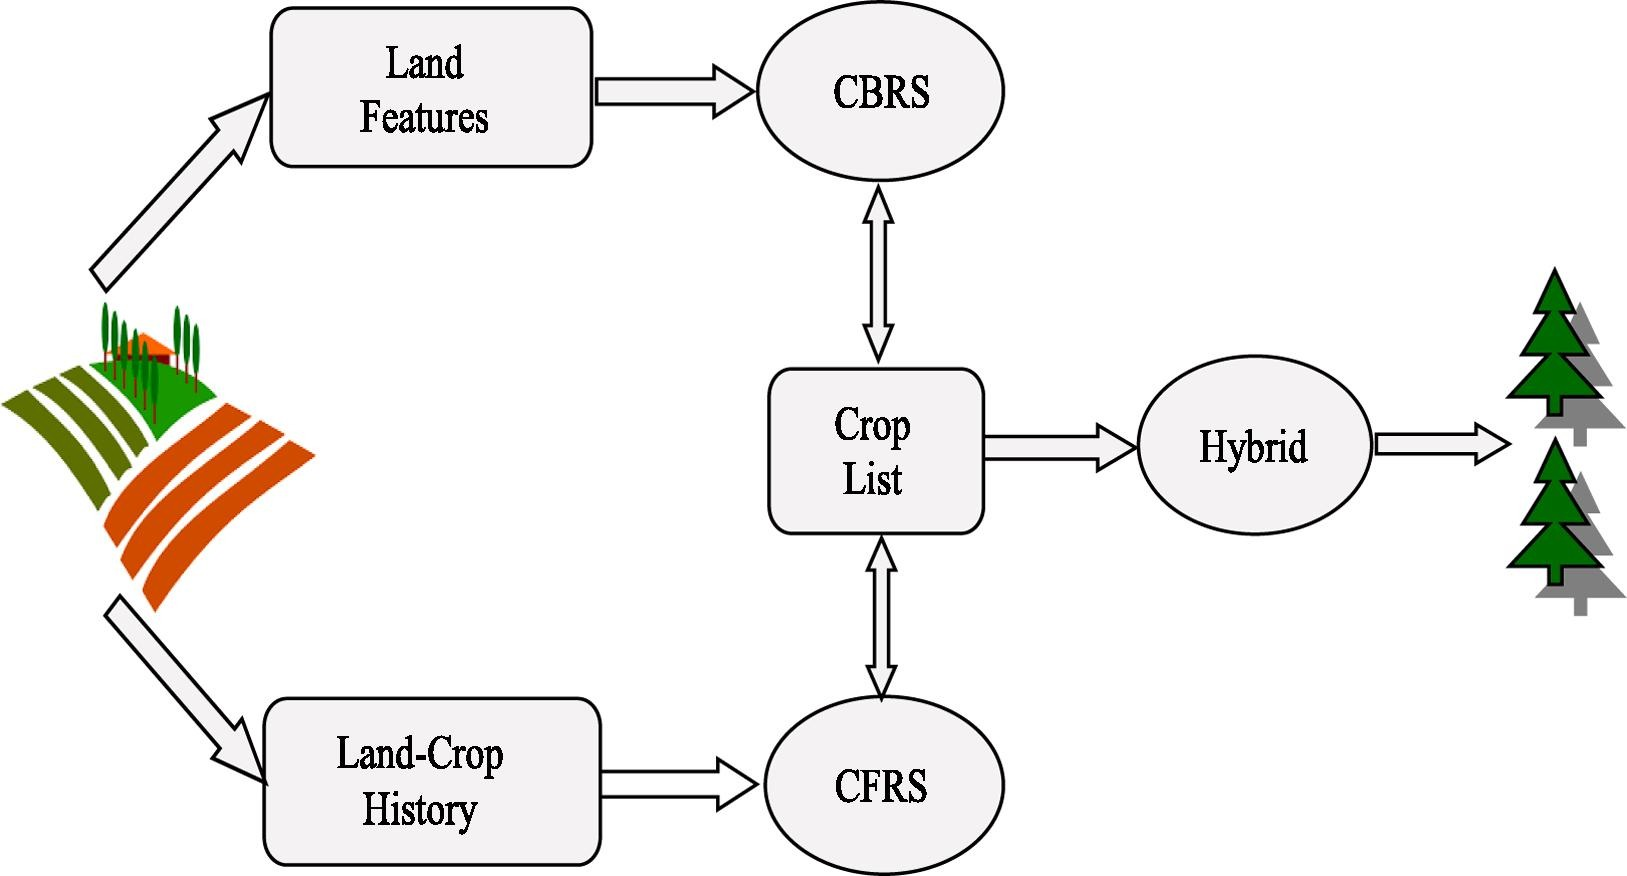
\includegraphics[width=\linewidth]{../graphics/Hybrid_RS_Land_Voorbeeld.jpg}
  \caption{Voorbeeld van hoe een hybride aanbevelingssysteem eruit kan zien \autocite{Patel2020}.} 
  \label{fig:hybrid_rs_land_voorbeeld}
\end{figure}

Het doel is een werkend proof-of-concept systeem te bouwen dat accurate en gepersonaliseerde aanbevelingen kan genereren, waarbij het vrijwel geen toegang heeft tot gevoelige gegevens van gebruikers. Door een combinatie van privacy behoudende technologieën, zoals FL en DP, vindt dit systeem een balans tussen bruikbaarheid en privacy. Als dit lukt, kan het een belangrijke stap zijn in de ontwikkeling van veilige en effectieve aanbevelingssystemen die vertrouwen winnen bij de gebruiker.

%---------- Stand van zaken ---------------------------------------------------
\section{Literatuurstudie}
\label{sec:literatuurstudie}

Aanbevelingssystemen zijn de laatste jaren enorm in opkomst en worden toegepast in verschillende sectoren. Ze zijn essentieel voor het bieden van gepersonaliseerde diensten aan gebruikers. Daarnaast vormen zulke diensten een effectieve inkomstenbron voor online bedrijven \autocite{Mazeh2020, Wang2018}. Echter, het gebruik van aanbevelingsdiensten vergt verzamelen van persoonlijke gegevens van gebruikers voor verwerking en analyse, wat gebruikers ongewenst vatbaar maakt voor privacyrisico's. Verder heeft elke serviceprovider een database met informatie over al zijn gebruikers \autocite{Wang2018, Lex2023, Yang2020, Friedman2015}.

Er zijn verschillende oplossingen uitgevonden om de privacy van gebruikers te beschermen. Eerste is Collaborative Filtering (CF), dit is een techniek die wordt gebruikt in aanbevelingssystemen om gebruikers te groeperen op basis van hun voorkeuren en interesses ten overzichte van andere gebruikers. Maar CF vereist een centrale server die de gegevens opslaat \autocite{Li2017,Wang2018}. Dit zorgt voor dat deze gebruikersgegevens kunnen worden misbruikt om privé informatie bekend te maken aan niet-vertrouwde partijen en om gebruikerskenmerken zoals geslacht of leeftijd af te leiden \autocite{Lex2023}. 
Differentional Privacy (DP) kan hierbij een oplossing bieden, uit \textcite{Friedman2015,Lex2023} volgt dat DP "is een rigoureus privacymodel dat ervoor zorgt dat de uitvoer van een berekening niet onthult of de gegevens van een specifieke persoon in de dataset zijn opgenomen". Dit wordt bereikt door zorgvuldig gekalibreerde ruis toe te voegen om de invloed van een enkele datapunt te maskeren.

Tweede techniek is Content Based (CB), aanbvelingssysteemen gebaseerd op CB bevelen items aan gebruikers aan op basis van de overeenkomsten tussen de inhoud van die items en voorkeuren van de gebruiker \autocite{Lops2010,Pazzani2007}. Hierbij worden verschillende datapunten van items en gebruikersprofielen geanalyseerd om patronen en voorkeuren te ontdekken en te groeperen. Hierin ligt ook het verschil met CF, waarbij de focus ligt op de overeenkomsten tussen gebruikers onderling. Nadelen van CB houden in: overspecialisatie, aanbevelingen hebben smal bereik van gebruikersinteresses, wat de ontdekking van nieuwe en diverse inhoud kan belemmeren en gedetailleerde analyse van gegevens, wat complex en tijdrovend kan zijn afhankelijk van de aard van de gegevens \autocite{Patel2020,Lops2010}.
In combinatie met Federated Learning (FL) kan CB verebterd worden. In plaats van gebruikersinformatie naar een centrale server te sturen, worden modellen getraind op het apparaat van de gebruikers zelf. Zo blijven persoonlijke gegevens lokaal bij de gebruiker en worden nooit uitgestuurd. Alleen geanonimiseerde modelupdates worden gedeeld met een centrale server, waardoor het systeem leert van de verzamelde inzichten zonder individuele gegevens te verzamelen \autocite{Wang2018, Lops2010}.

% Voor literatuurverwijzingen zijn er twee belangrijke commando's:
% \autocite{KEY} => (Auteur, jaartal) Gebruik dit als de naam van de auteur
%   geen onderdeel is van de zin.
% \textcite{KEY} => Auteur (jaartal)  Gebruik dit als de auteursnaam wel een
%   functie heeft in de zin (bv. ``Uit onderzoek door Doll & Hill (1954) bleek
%   ...'')

%---------- Methodologie ------------------------------------------------------
%// [ ] hoe wil ik DE en FL combineren 
%// [ ] tijdschatting gantt diagram opstellen, zie RM

\section{Methodologie}%
\label{sec:methodologie}

We passen het strtegie van verdeel en heers om dit probleem makkelijker op te lossen. Beschouw het hybride aanbevelingssysteem als een combinatie van twee subsystemen: een Content Based (CB) gebaseerde en Collaborative Filtering (CF) gebaseerde systeem. 

Hier beschrijf je hoe je van plan bent het onderzoek te voeren. Welke onderzoekstechniek ga je toepassen om elk van je onderzoeksvragen te beantwoorden? Gebruik je hiervoor literatuurstudie, interviews met belanghebbenden (bv.~voor requirements-analyse), experimenten, simulaties, vergelijkende studie, risico-analyse, PoC, \ldots?

Valt je onderwerp onder één van de typische soorten bachelorproeven die besproken zijn in de lessen Research Methods (bv.\ vergelijkende studie of risico-analyse)? Zorg er dan ook voor dat we duidelijk de verschillende stappen terug vinden die we verwachten in dit soort onderzoek!

Vermijd onderzoekstechnieken die geen objectieve, meetbare resultaten kunnen opleveren. Enquêtes, bijvoorbeeld, zijn voor een bachelorproef informatica meestal \textbf{niet geschikt}. De antwoorden zijn eerder meningen dan feiten en in de praktijk blijkt het ook bijzonder moeilijk om voldoende respondenten te vinden. Studenten die een enquête willen voeren, hebben meestal ook geen goede definitie van de populatie, waardoor ook niet kan aangetoond worden dat eventuele resultaten representatief zijn.

Uit dit onderdeel moet duidelijk naar voor komen dat je bachelorproef ook technisch voldoen\-de diepgang zal bevatten. Het zou niet kloppen als een bachelorproef informatica ook door bv.\ een student marketing zou kunnen uitgevoerd worden.

Je beschrijft ook al welke tools (hardware, software, diensten, \ldots) je denkt hiervoor te gebruiken of te ontwikkelen.

Probeer ook een tijdschatting te maken. Hoe lang zal je met elke fase van je onderzoek bezig zijn en wat zijn de concrete \emph{deliverables} in elke fase?

%---------- Verwachte resultaten ----------------------------------------------
\section{Verwacht resultaat, conclusie}%
\label{sec:verwachte_resultaten}

Hier beschrijf je welke resultaten je verwacht. Als je metingen en simulaties uitvoert, kan je hier al mock-ups maken van de grafieken samen met de verwachte conclusies. Benoem zeker al je assen en de onderdelen van de grafiek die je gaat gebruiken. Dit zorgt ervoor dat je concreet weet welk soort data je moet verzamelen en hoe je die moet meten.

Wat heeft de doelgroep van je onderzoek aan het resultaat? Op welke manier zorgt jouw bachelorproef voor een meerwaarde?

Hier beschrijf je wat je verwacht uit je onderzoek, met de motivatie waarom. Het is \textbf{niet} erg indien uit je onderzoek andere resultaten en conclusies vloeien dan dat je hier beschrijft: het is dan juist interessant om te onderzoeken waarom jouw hypothesen niet overeenkomen met de resultaten.

